\documentclass[tikz,border=20pt]{standalone}
\usepackage{tikz}
\usepackage{amsmath,amssymb}
\usetikzlibrary{arrows.meta, decorations.markings, backgrounds, calc}

% ── Colours ──────────────────────────────────────────────────────────
\definecolor{evbg}     {RGB}{228,236,255}
\definecolor{evbd}     {RGB}{ 55, 85,175}
\definecolor{brev}     {RGB}{195, 65, 25}
\definecolor{facefill} {RGB}{255,212, 60}
\definecolor{l2col}    {RGB}{ 35,135, 70}
\definecolor{holcol}   {RGB}{155, 25, 20}
\definecolor{voidcol}  {RGB}{0,0,0}
\definecolor{panelbg}  {RGB}{251,251,254}
\definecolor{panelbd}  {RGB}{100,100,110}   % darker panel border
\definecolor{chargecol}{RGB}{155, 35,165}

% ── Styles ───────────────────────────────────────────────────────────
\tikzset{
  evbox/.style={
    rectangle, rounded corners=5pt,
    draw=evbd, fill=evbg, line width=1.1pt,
    minimum width=3.2cm, minimum height=0.85cm,
  font=\small, inner sep=5pt, align=center},
  brevbox/.style={evbox, draw=brev, fill=brev!10},
  voidbox/.style={evbox, draw=voidcol, fill=voidcol!8,
  text=voidcol, dashed},
  carr/.style={->, evbd,  line width=1.1pt, >=Stealth},
  barr/.style={->, brev,  line width=1.1pt, >=Stealth, dashed},
  l2n/.style={circle, draw=evbd, fill=white, line width=1.2pt,
  minimum size=9mm, font=\small\bfseries, inner sep=0pt},
  l2v/.style={l2n, draw=voidcol, text=voidcol, dashed},
  l2t/.style={l2col,  line width=2.0pt},
  l2b/.style={brev,   line width=2.0pt, dashed},
  nbadge/.style={font=\scriptsize, evbd,
    fill=white, draw=evbd!50,
  rounded corners=2pt, inner sep=2pt},
  cbadge/.style={font=\scriptsize\bfseries, chargecol,
    fill=white, draw=chargecol,
  rounded corners=2pt, inner sep=2pt},
  vbadge/.style={font=\scriptsize\bfseries, voidcol,
    fill=white, draw=voidcol, dashed,
  rounded corners=2pt, inner sep=2pt},
  elab/.style={font=\scriptsize\bfseries,
  fill=panelbg, inner sep=1.5pt, rounded corners=1pt},
  phdr/.style={font=\small\bfseries, fill=white,
    draw=panelbd, rounded corners=4pt,
  line width=0.9pt, inner sep=6pt}
}

\begin{document}
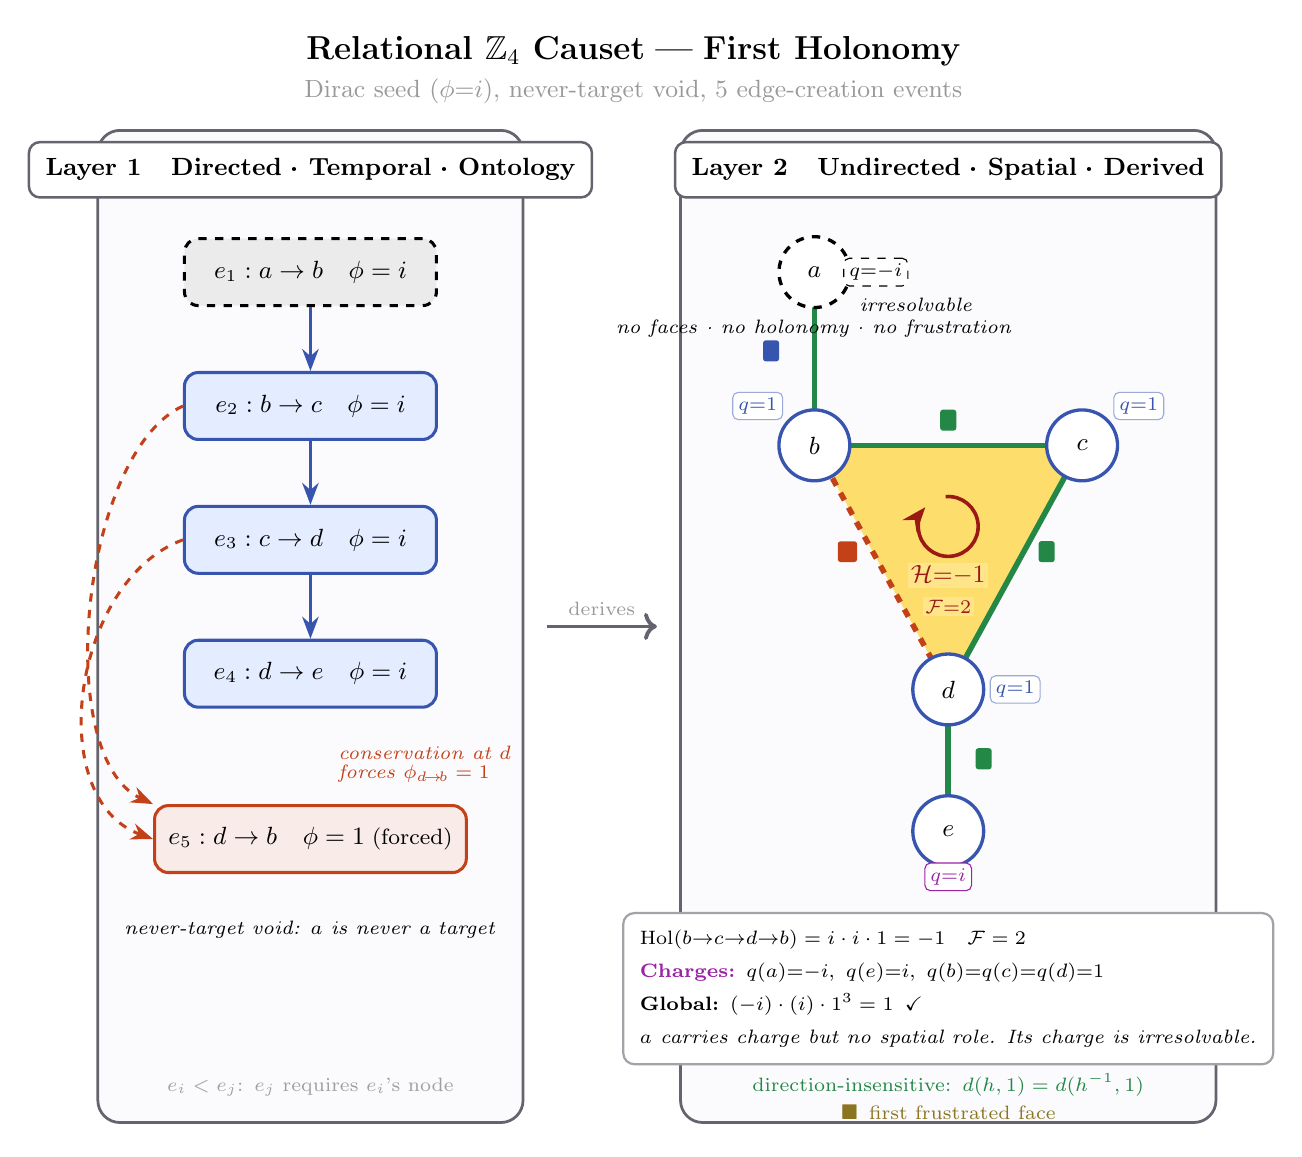
\begin{tikzpicture}

  % ================================================================
  %  Global title
  % ================================================================
  \node[font=\large\bfseries] at (6.8, 13.6)
  {Relational $\mathbb{Z}_4$ Causet\;---\;First Holonomy};
  \node[font=\small, gray!80] at (6.8, 13.1)
  {Dirac seed ($\phi{=}i$), never-target void, 5 edge-creation events};

  % ================================================================
  %  LAYER 1   panel: (0,0)–(5.4,12.6)
  % ================================================================
  \begin{scope}

    \fill[panelbg, rounded corners=8pt] (0,0) rectangle (5.4,12.6);
    \draw[panelbd, rounded corners=8pt, line width=1.0pt]
    (0,0) rectangle (5.4,12.6);
    \node[phdr] at (2.7, 12.1)
    {\textbf{Layer 1}\quad Directed · Temporal · Ontology};

    % event boxes centred at x=2.7
    \node[voidbox] (e1) at (2.7, 10.8)
    {$e_1 : a \to b \quad \phi = i$};
    \node[evbox]   (e2) at (2.7,  9.1)
    {$e_2 : b \to c \quad \phi = i$};
    \node[evbox]   (e3) at (2.7,  7.4)
    {$e_3 : c \to d \quad \phi = i$};
    \node[evbox]   (e4) at (2.7,  5.7)
    {$e_4 : d \to e \quad \phi = i$};
    \node[brevbox] (e5) at (2.7,  3.6)
    {$e_5 : d \to b \quad \phi = 1$\;{\footnotesize(forced)}};

    % straight causal arrows
    \draw[carr] (e1) -- (e2);
    \draw[carr] (e2) -- (e3);
    \draw[carr] (e3) -- (e4);

    % bridge arrows: left side, controlled to stay inside panel
    \draw[barr] (e3.west) to[out=200, in=160, looseness=1.0] (e5.west);
    \draw[barr] (e2.west) to[out=205, in=155, looseness=0.72] (e5.north west);

    % conservation note — right of e5, well inside panel
    \node[font=\scriptsize, brev, align=left] at (4.15, 4.55)
    {\textit{conservation at $d$}\\[-1pt]
    \textit{forces $\phi_{d\!\to\! b}=1$}};

    % void note
    \node[font=\scriptsize, voidcol, align=center] at (2.7, 2.45)
    {\textit{never-target void: $a$ is never a target}};

    % ordering note
    \node[font=\scriptsize, gray!75, align=center] at (2.7, 0.45)
    {$e_i < e_j$:\enspace $e_j$ requires $e_i$'s node};

  \end{scope}

  % ================================================================
  %  derives arrow
  % ================================================================
  \draw[->, panelbd, line width=1.4pt]
  (5.7, 6.3) -- (7.1, 6.3)
  node[midway, above, font=\scriptsize, gray!80] {derives};

  % ================================================================
  %  LAYER 2   panel: (7.4,0)–(14.2,12.6)
  %
  %  Triangle b–c–d centroid at (10.8, 7.0):
  %    b = (9.1, 8.6)   top-left
  %    c = (12.5, 8.6)  top-right
  %    d = (10.8, 5.5)  bottom
  %  Centroid = ((9.1+12.5+10.8)/3, (8.6+8.6+5.5)/3) = (10.8, 7.57)
  %  Holonomy arc: small circle radius 0.38 at centroid (3.4, 7.57) in scope
  %
  %  In scope coords (xshift=7.4):
  %    Na = (1.7, 10.8)   void a
  %    Nb = (1.7,  8.6)   b
  %    Nc = (5.1,  8.6)   c
  %    Nd = (3.4,  5.5)   d
  %    Ne = (3.4,  3.7)   e
  %  Centroid of b–c–d = (3.4, 7.57)
  % ================================================================
  \begin{scope}[xshift=7.4cm]

    \fill[panelbg, rounded corners=8pt] (0,0) rectangle (6.8,12.6);
    \draw[panelbd, rounded corners=8pt, line width=1.0pt]
    (0,0) rectangle (6.8,12.6);
    \node[phdr] at (3.4, 12.1)
    {\textbf{Layer 2}\quad Undirected · Spatial · Derived};

    % coordinates
    \coordinate (Na) at (1.7, 10.8);
    \coordinate (Nb) at (1.7,  8.6);
    \coordinate (Nc) at (5.1,  8.6);
    \coordinate (Nd) at (3.4,  5.5);
    \coordinate (Ne) at (3.4,  3.7);
    % face centroid
    \coordinate (Ctr) at (3.4, 7.57);

    % face fill
    \fill[facefill, opacity=0.75] (Nb) -- (Nc) -- (Nd) -- cycle;

    % edges
    \draw[l2t] (Na) -- (Nb);
    \draw[l2t] (Nb) -- (Nc);
    \draw[l2t] (Nc) -- (Nd);
    \draw[l2t] (Nd) -- (Ne);
    \draw[l2b] (Nd) -- (Nb);

    % edge phase labels — all outside the triangle or on the a–b edge
    \node[elab, evbd]  at (1.15, 9.8)  {$i$};    % a–b left
    \node[elab, l2col] at (3.4,  8.92) {$i$};    % b–c above
    \node[elab, l2col] at (4.65, 7.25) {$i$};    % c–d right outside
    \node[elab, l2col] at (3.85, 4.62) {$i$};    % d–e right
    \node[elab, brev]  at (2.12, 7.25) {$1$};    % d–b left outside

    % holonomy traversal arrow — small arc at centroid, clear of all edges
    % radius 0.38, clockwise from top: start 95°, sweep to −220° (=−220)
    \draw[->, holcol, line width=1.3pt, >=Stealth]
    ($(Ctr)+(95:0.38)$)
    arc[start angle=95, end angle=-220, radius=0.38];

    % holonomy label — below the arc, still inside face
    \node[holcol, font=\small\bfseries, fill=facefill!60, inner sep=1pt]
    at ($(Ctr)+(0,-0.62)$) {$\mathcal{H}{=}{-1}$};
    \node[holcol, font=\scriptsize, fill=facefill!60, inner sep=1pt]
    at ($(Ctr)+(0,-1.02)$) {$\mathcal{F}{=}2$};

    % ── void node a ───────────────────────────────────────────────
    % node itself
    \node[l2v] (Av) at (Na) {$a$};
    % charge badge: right of node
    \node[vbadge] at ($(Na)+(0.78, 0.0)$) {$q{=}{-i}$};
    % "irresolvable" — right, below badge
    \node[font=\scriptsize\itshape, voidcol, anchor=west]
    at ($(Na)+(0.45,-0.42)$) {irresolvable};
    % spatial note — below node, centred
    \node[font=\scriptsize, voidcol, align=center]
    at ($(Na)+(0.0,-0.72)$)
    {\textit{no faces · no holonomy · no frustration}};

    % ── nodes b, c, d, e ──────────────────────────────────────────
    \node[l2n] at (Nb) {$b$};
    \node[nbadge] at ($(Nb)+(-0.72, 0.50)$) {$q{=}1$};

    \node[l2n] at (Nc) {$c$};
    \node[nbadge] at ($(Nc)+(0.72, 0.50)$) {$q{=}1$};

    \node[l2n] at (Nd) {$d$};
    \node[nbadge] at ($(Nd)+(0.85, 0.0)$) {$q{=}1$};

    \node[l2n] at (Ne) {$e$};
    \node[cbadge] at ($(Ne)+(0.0,-0.58)$) {$q{=}i$};

    % ── summary box ───────────────────────────────────────────────
    \node[font=\scriptsize, align=left,
      fill=white, draw=panelbd!60, rounded corners=4pt,
    line width=0.8pt, inner sep=6pt] at (3.4, 1.7)
    {$\mathrm{Hol}(b{\to}c{\to}d{\to}b)
      = i\cdot i\cdot 1 = -1$\quad$\mathcal{F}=2$\\[4pt]
      \textcolor{chargecol}{\textbf{Charges:}}\enspace
      $q(a){=}{-i}$,\enspace $q(e){=}{i}$,\enspace
      $q(b){=}q(c){=}q(d){=}1$\\[4pt]
      \textbf{Global:}\enspace
      $({-i})\cdot(i)\cdot 1^3 = 1$\enspace\checkmark\\[4pt]
      \textcolor{voidcol}{\textit{%
          $a$ carries charge but no spatial role.
    Its charge is irresolvable.}}};

    % footnotes
    \node[font=\scriptsize, l2col, align=center] at (3.4, 0.48)
    {direction-insensitive:\enspace $d(h,1)=d(h^{-1},1)$};
    \node[font=\scriptsize, facefill!55!black] at (3.4, 0.13)
    {$\blacksquare$\enspace first frustrated face};

  \end{scope}

\end{tikzpicture}
\end{document}
